\documentclass{article}
\usepackage{graphicx}
\usepackage{caption}
\usepackage{float} % for H specifier

\begin{document}
\title{\textbf{Analog IC Lab \#1}}
\date{} % Remove date
\author{{Hatem Mohamed Ahmed Rashed}{	20010447} \\
{Ziad Amr Ibrahim Mohamed}{	20010637} }
\maketitle
	%=================================================================%
	%                       PART 2
	%=================================================================%

	\section{Practical Results}
	%===========================PLOT==================================%
	\subsection{Unity Gain Amplifier}
	\begin{figure}[H]
		\centering
		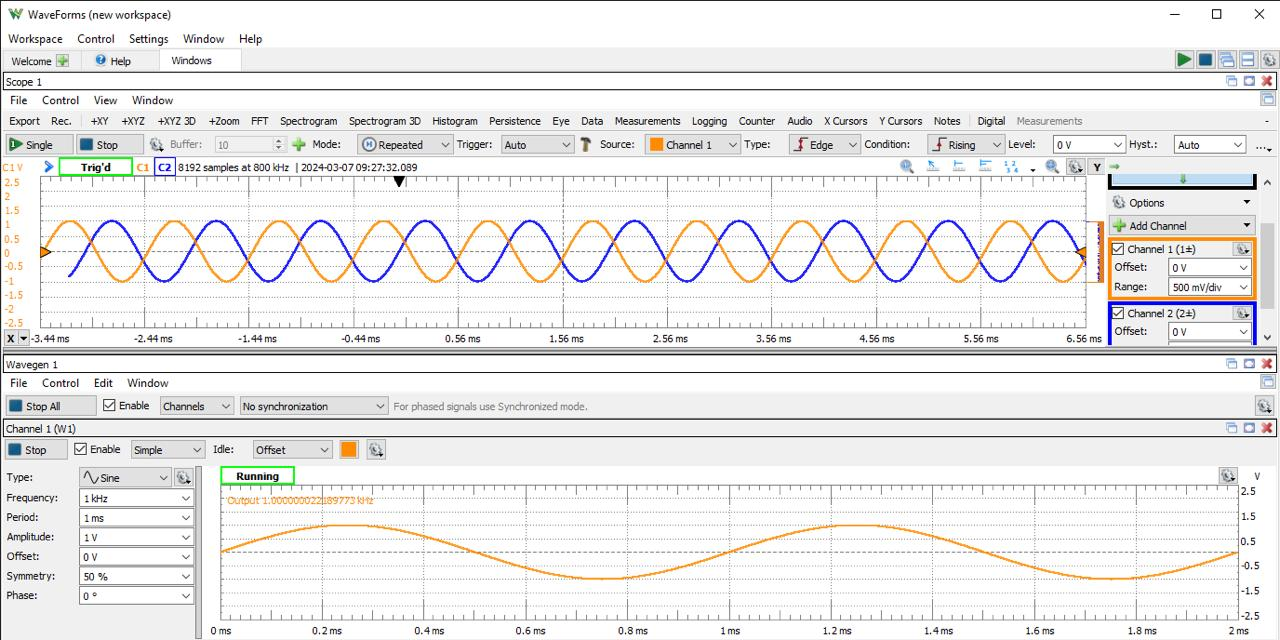
\includegraphics[width=1\textwidth]{unity_gain.jpg}
		\caption{The prictical result plot for Unity Gain Amplifier}
		\label{fig:practiacal_unity}
	\end{figure}
	%===========================PLOT==================================%
	\subsection{Non Inverting Amplifier with Gain of 2}
	\begin{figure}[H]
		\centering
		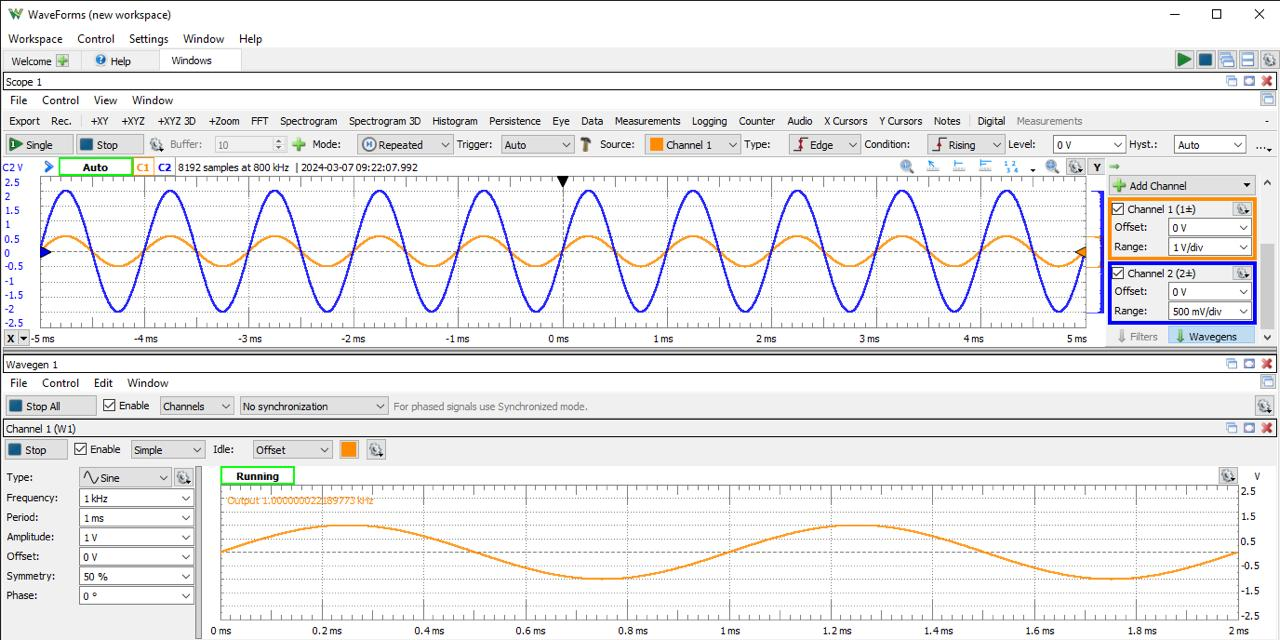
\includegraphics[width=1\textwidth]{gain_2.jpg}
		\caption{The prictical result plot for Non Inverting Amplifier with Gain of 2}
		\label{fig:2Gain}
	\end{figure}
	%===========================PLOT==================================%
	
	%===========================PLOT==================================%
	\subsection{Inverting Amplifier with Gain of 2.2}
	\begin{figure}[H]
		\centering
		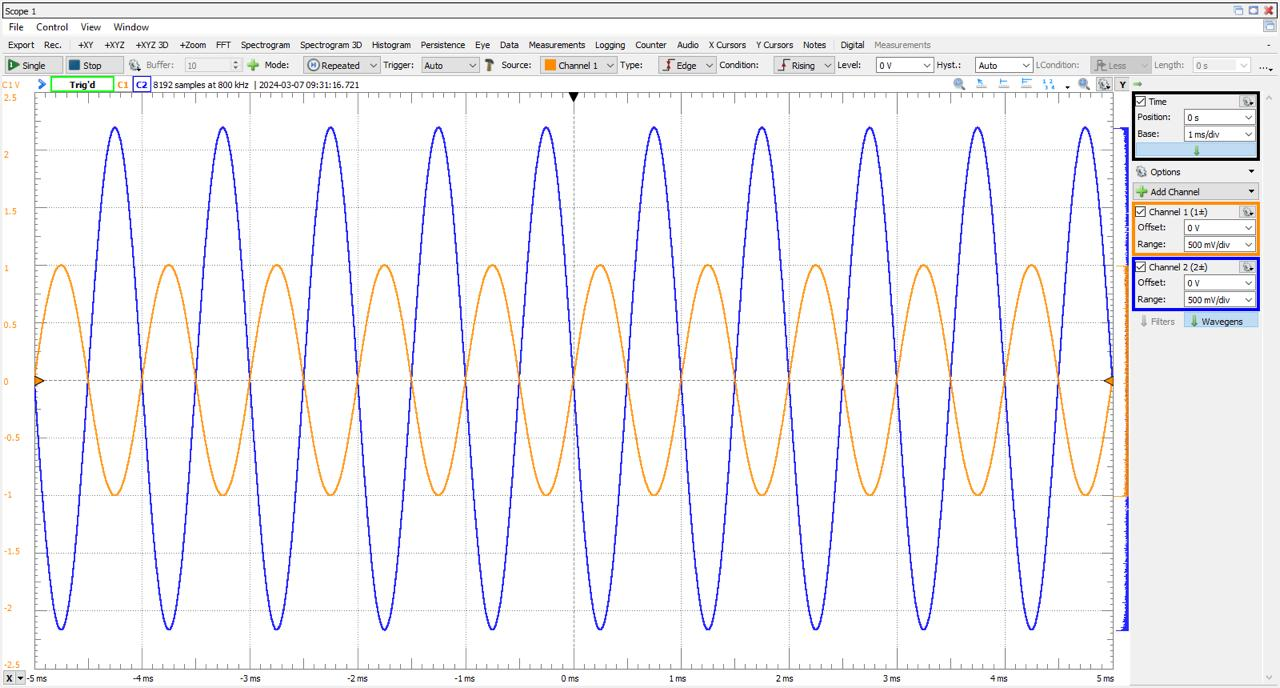
\includegraphics[width=1\textwidth]{gain2_4.jpg}
		\caption{The prictical result plot for Inverting Amplifier with Gain of 2.2}
		\label{fig:2_4Gain}
	\end{figure}

	%=================================================================%
	%                       PART 2
	%=================================================================%
	
	\section{Simulation Results}
	%=================================================================%
	%                       TYPE1
	%=================================================================%
	
	
	%===========================PLOT==================================%
	\subsection{Unity Gain Amplifier}
	\subsubsection{Unity Sine Gain}
	\begin{figure}[H]
		\centering
		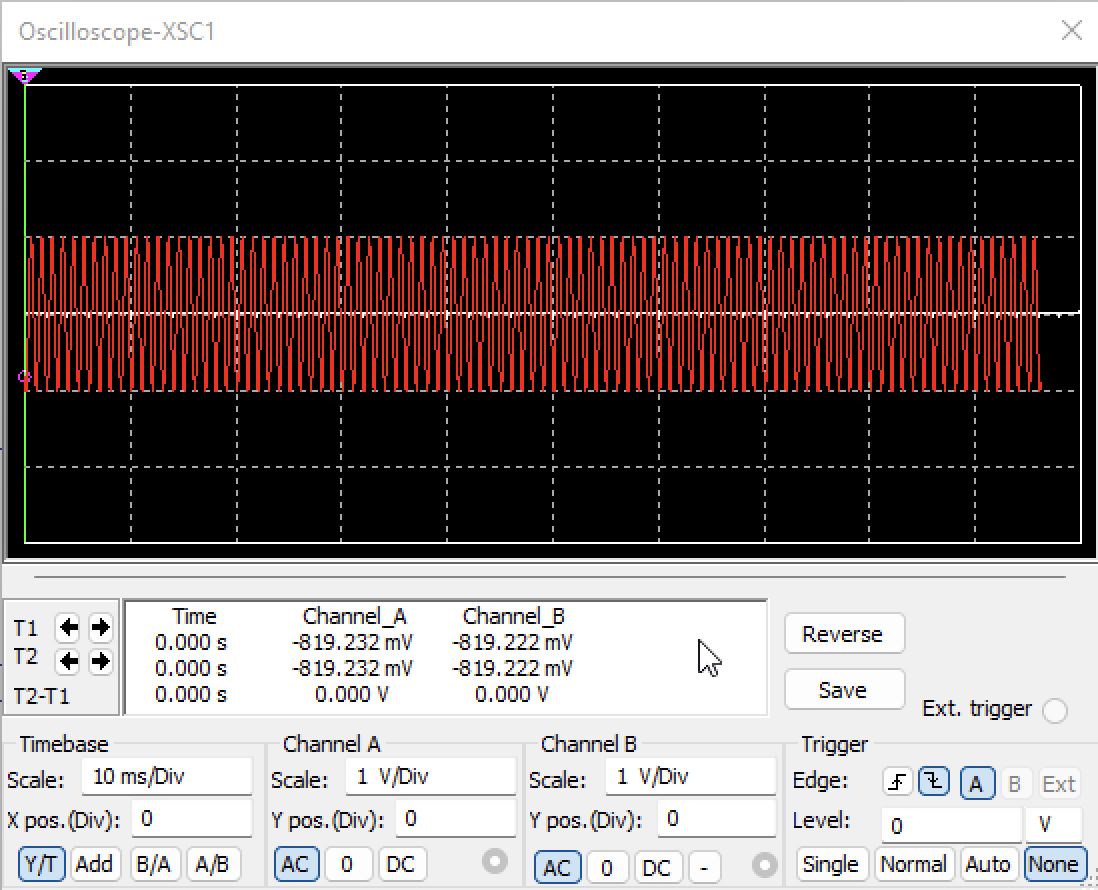
\includegraphics[width=1\textwidth]{Unity/UnitySineGain.png}
		\caption{The simulation plot for Unity Sine Gain}
		\label{fig:UnitySineGain}
	\end{figure}
	%===========================PLOT==================================%
	\subsubsection{Unity Sine Frequency}
	\begin{figure}[H]
	\centering
	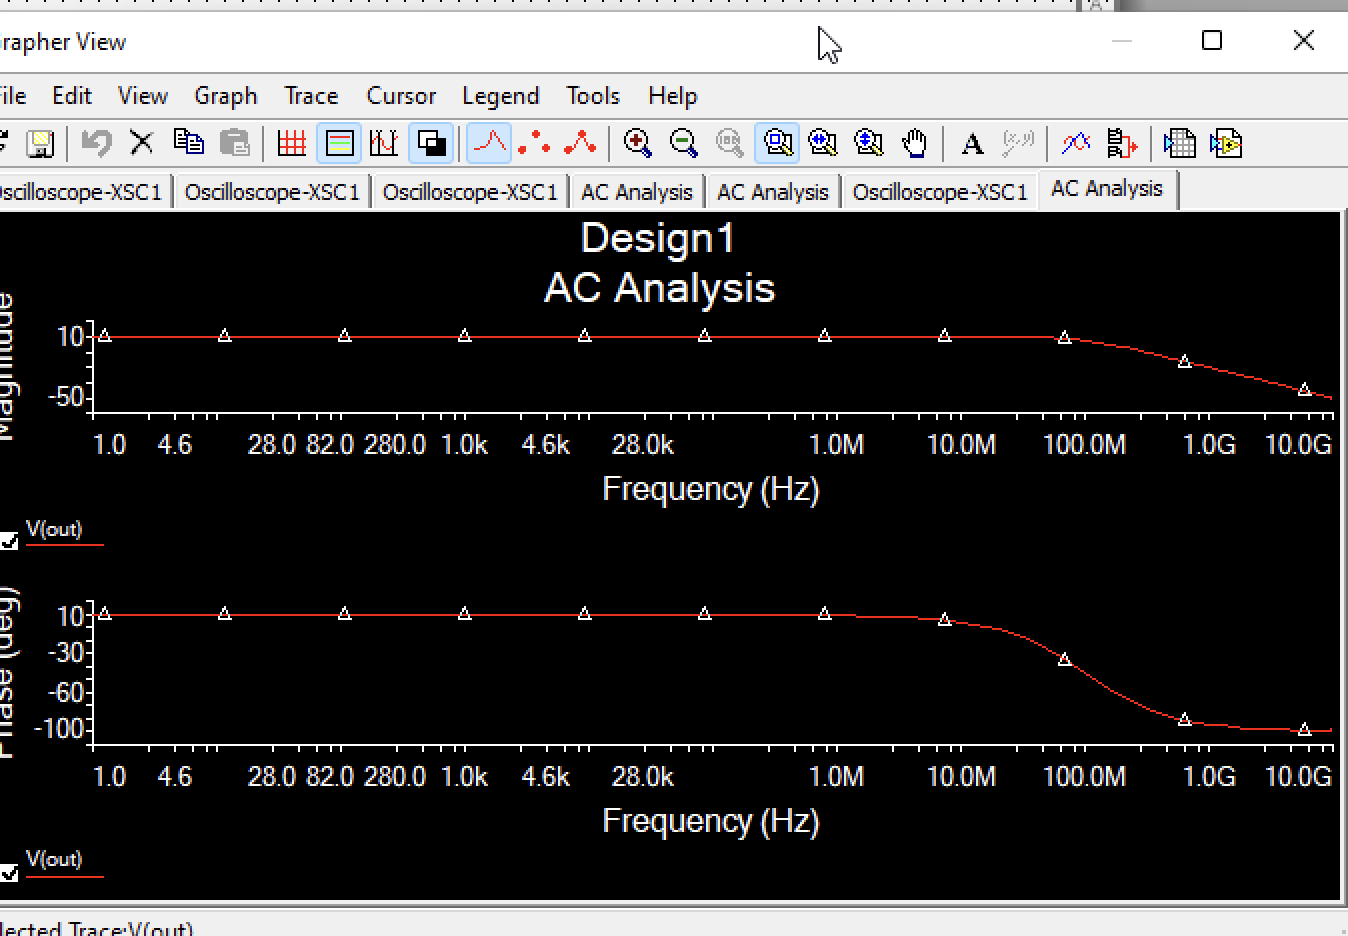
\includegraphics[width=1\textwidth]{Unity/UnitySineFreq.png}
	\caption{The simulation plot for Unity Sine Freq}
	\label{fig:UnitySineFreq}
	\end{figure}
	%===========================PLOT==================================%
	
	%===========================PLOT==================================%
	\subsubsection{Unity Square Gain}
	\begin{figure}[H]
	\centering
	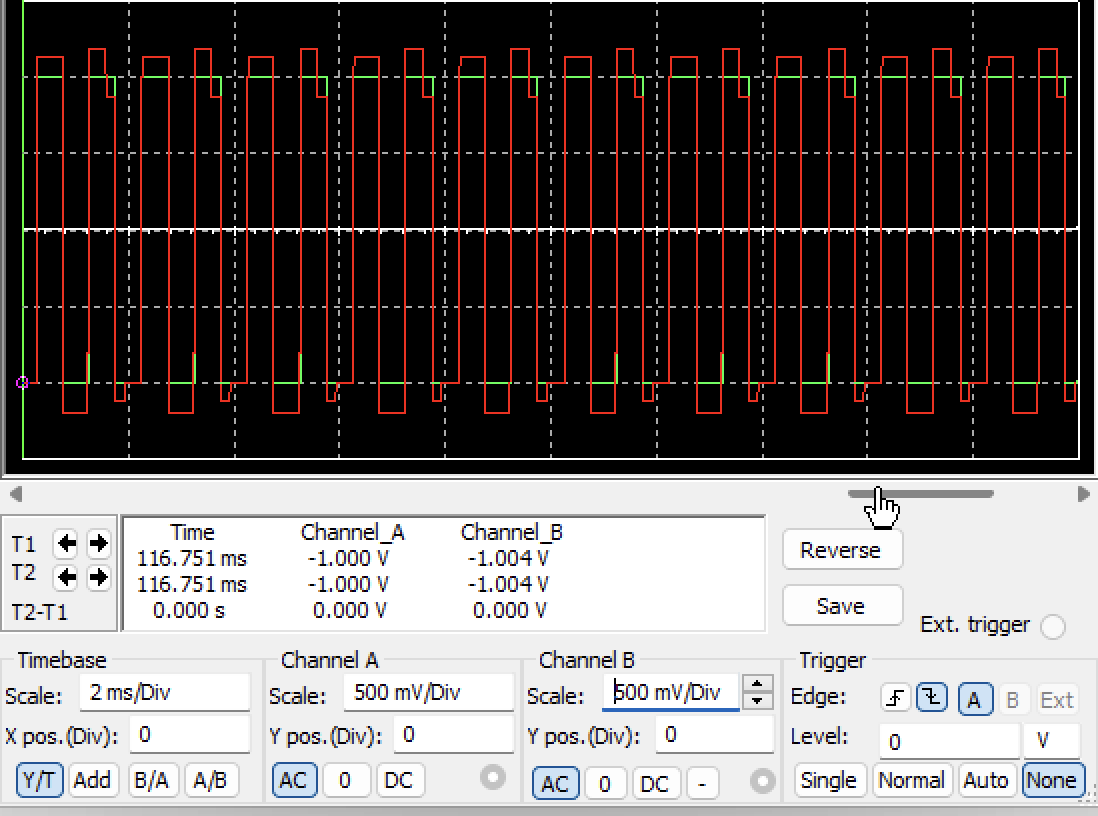
\includegraphics[width=1\textwidth]{Unity/UnitySquareGain.png}
	\caption{The simulation plot for unity Unity Square Gain}
	\label{fig:UnitySquareGain}
	\end{figure}
	%===========================PLOT==================================%
	
	\subsubsection{Unity Square Frequency}
	\begin{figure}[H]
	\centering
	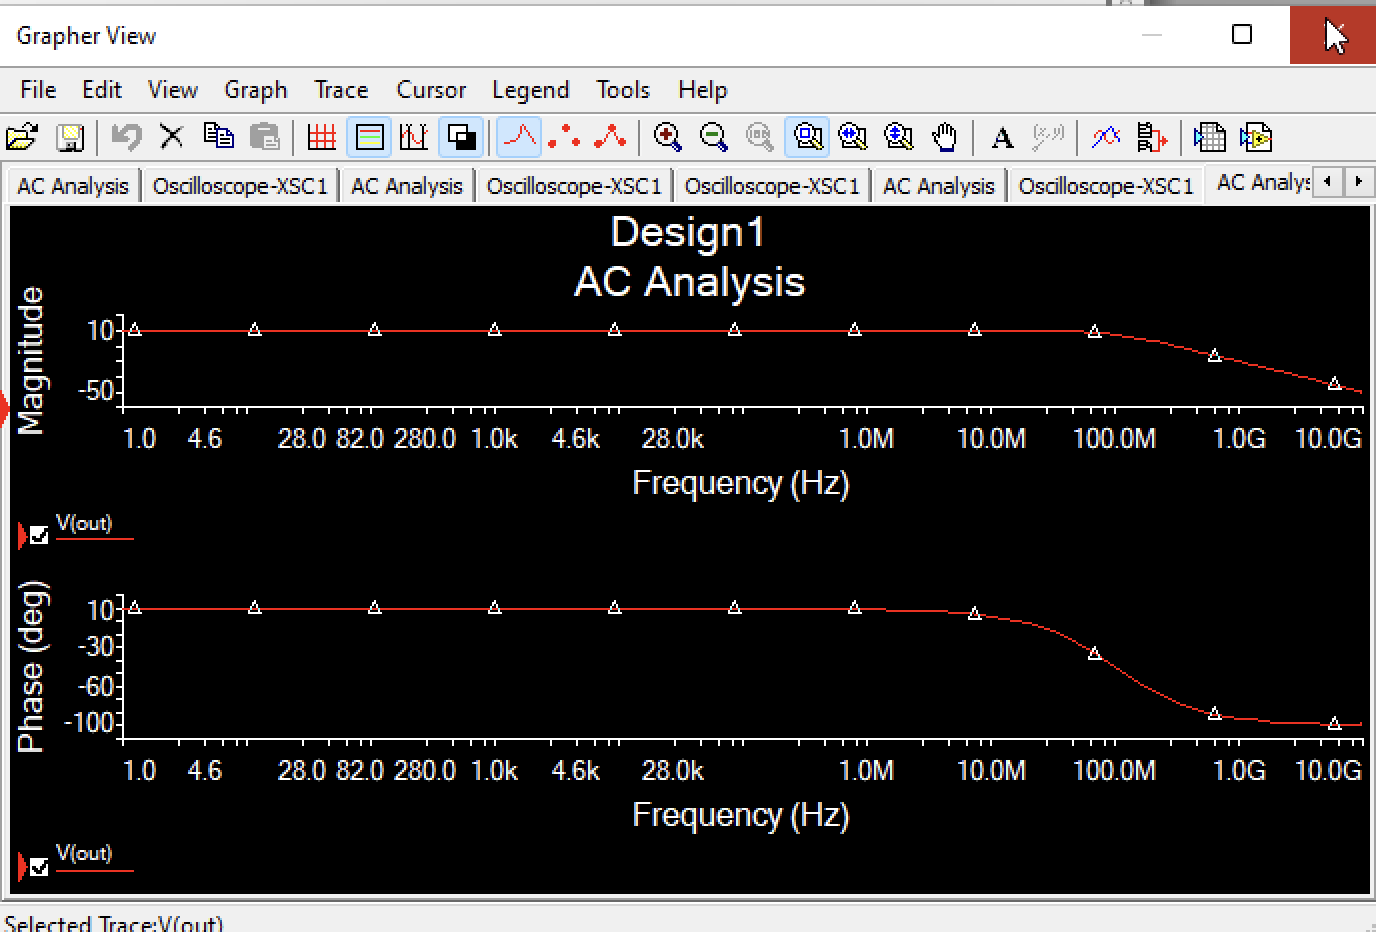
\includegraphics[width=1\textwidth]{Unity/UnitySquareFreq.png}
	\caption{The simulation plot for Unity Square Freq}
	\label{fig:UnitySquareFreq}
	\end{figure}
	%===========================END TYPE 1============================%
	
	
	%=================================================================%
	%                       TYPE2
	%=================================================================%
	
	
	%===========================PLOT==================================%
	\subsection{Non Inverting Amplifier}
	\subsubsection{Non Inverting Amplifier Circuit}
	\begin{figure}[H]
	
	\centering
	\includegraphics[width=1\textwidth]{"Non Inverting"/circuit.png}
	\caption{The simulation plot for Non Inverting Amplifier circuit}
	\label{fig:non_inv_circuit}
	\end{figure}
	%===========================PLOT==================================%
	\subsubsection{Non Inverting Amplifier Sine Gain}
	\begin{figure}[H]
	
	\centering
	\includegraphics[width=1\textwidth]{"Non Inverting"/sine_gain.png}
	\caption{The simulation plot for Non Inverting Amplifier Sine Gain}
	\label{fig:noninv_sine_gain}
	\end{figure}
	%===========================PLOT==================================%
	\subsubsection{Non Inverting Amplifier Sine Frequency}
	\begin{figure}[H]
	
	\centering
	\includegraphics[width=1\textwidth]{"Non Inverting"/Sine.png}
	\caption{The simulation plot for Non Inverting Amplifier Square Gain}
	\label{fig:noninv_SineFreq}
	\end{figure}
	%===========================PLOT==================================%
	
	%===========================PLOT==================================%
	\subsubsection{Non Inverting Amplifier Square Gain}
	\begin{figure}[H]
	
	\centering
	\includegraphics[width=1\textwidth]{"Non Inverting"/square_gain.png}
	\caption{The simulation plot for Non Inverting Amplifier Square Gain}
	\label{fig:noninv_square_gain}
	\end{figure}
	%===========================PLOT==================================%
	
	\subsubsection{Non Inverting Amplifier Square Frequency}
	\begin{figure}[H]
	
	\centering
	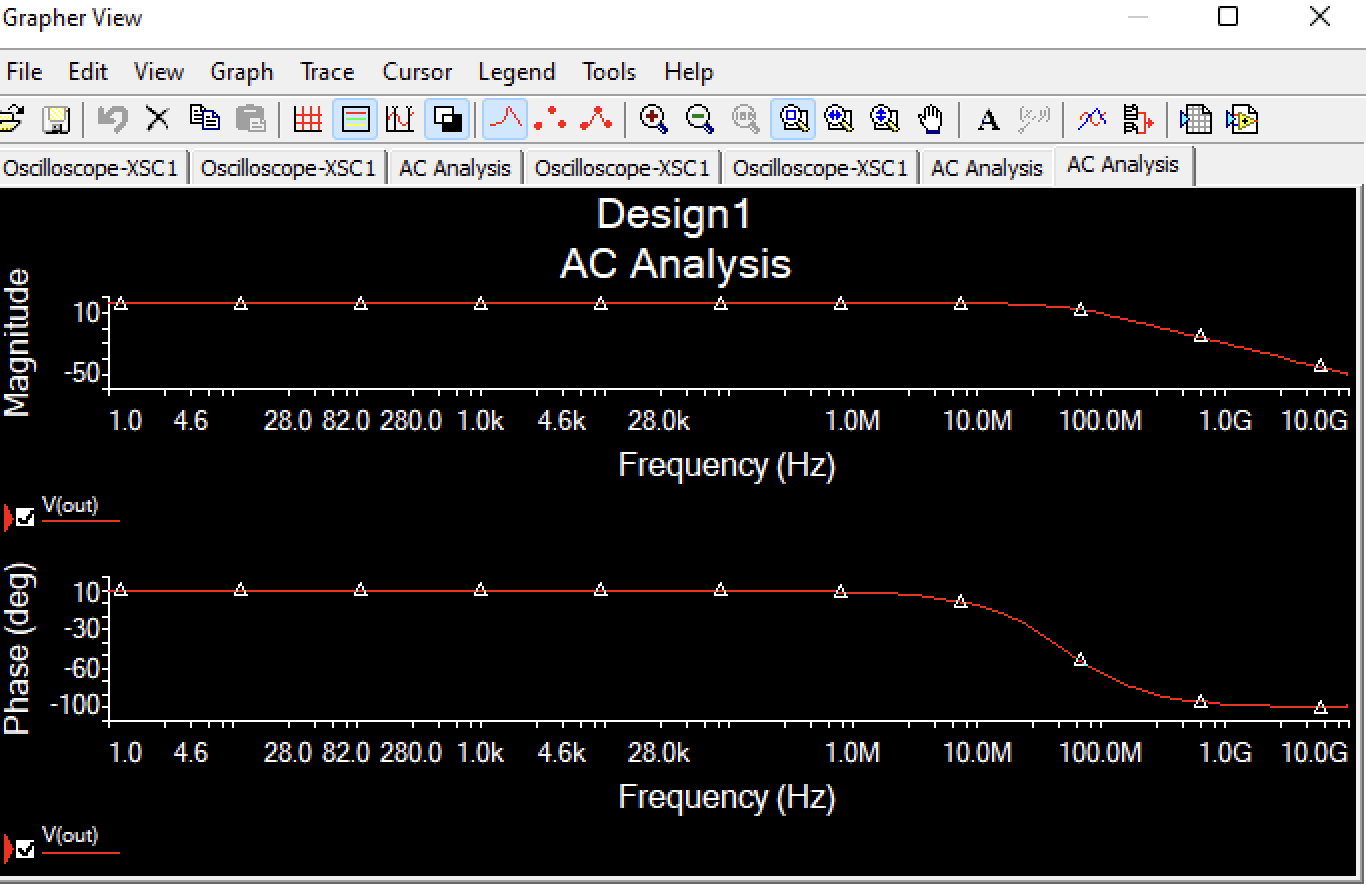
\includegraphics[width=1\textwidth]{"Non Inverting"/Rec.png}
	\caption{The simulation plot for Non Inverting Amplifier Square Frequency}
	\label{fig:noninv_SquareFreq}
	\end{figure}
	%===========================END TYPE 2============================%
	
	
	%=================================================================%
	%                       TYPE3
	%=================================================================%
	
	%===========================PLOT==================================%
	\subsection{Inverting Amplifier}
	\subsubsection{Inverting Amplifier Circuit}
	\begin{figure}[H]
	
	\centering
	\includegraphics[width=1\textwidth]{"Inverting"/circuit.png}
	\caption{The simulation plot for Inverting Amplifier circuit}
	\label{fig:inv_circuit}
	\end{figure}
	%===========================PLOT==================================%
	\subsubsection{Inverting Amplifier Sine Gain}
	\begin{figure}[H]
	
	\centering
	\includegraphics[width=1\textwidth]{"Inverting"/sine_gain.png}
	\caption{The simulation plot for Inverting Amplifier Sine Gain}
	\label{fig:inv_sine_gain}
	\end{figure}
	%===========================PLOT==================================%
	\subsubsection{Inverting Amplifier Sine Frequency}
	\begin{figure}[H]
	
	\centering
	\includegraphics[width=1\textwidth]{"Inverting"/Sine.png}
	\caption{The simulation plot for Inverting Amplifier Square Gain}
	\label{fig:inv_SineFreq}
	\end{figure}
	%===========================PLOT==================================%
	
	%===========================PLOT==================================%
	\subsubsection{Inverting Amplifier Square Gain}
	\begin{figure}[H]
	
	\centering
	\includegraphics[width=1\textwidth]{"Inverting"/square_gain.png}
	\caption{The simulation plot for Inverting Amplifier Square Gain}
	\label{fig:inv_square_gain}
	\end{figure}
	%===========================PLOT==================================%
	\subsubsection{Inverting Amplifier Square Frequency}
	
	\begin{figure}[H]
	
	\centering
	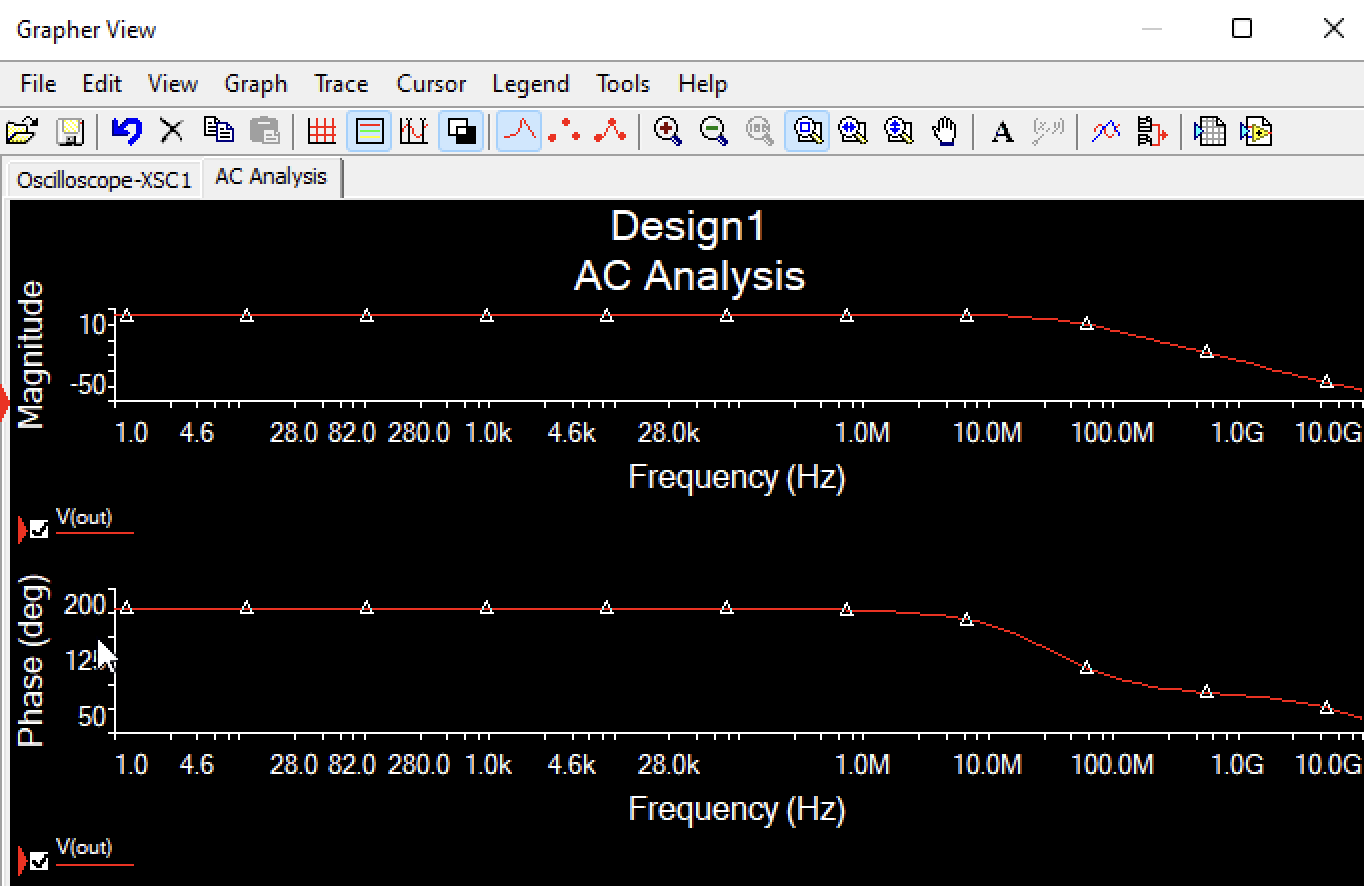
\includegraphics[width=1\textwidth]{"Inverting"/Square.png}
	\caption{The simulation plot for Inverting Amplifier Square Frequency}
	\label{fig:inv_SquareFreq}
	\end{figure}
	%===========================END TYPE 3============================%
	
	
	%=================================================================%
	%                       PART 2
	%=================================================================%
	
	
	\section{Instrumentation Amplifier}
	%=================================================================%
	%                       TYPE1
	%=================================================================%
	\subsection{instrumentation Amplifier with gain of 3}
	\subsubsection{Procedures}
	
	the procedures taken for this experment are to get a gain of 3
	\begin{equation}
	V{_{input1}} = 1 { volt}, \quad {Freq}{_{input1}} = 1 {kHz}
	\end{equation}
	
	\begin{equation}
	V{_{input2}} = 1.5 { volt}, \quad {Freq}{_{input2}} = 1 {kHz}
	\end{equation}
	
	\begin{equation}
	A_{v} = \left(1 + \frac{2 R}{R * n}\right) *\frac{R}{R} = 3
	\end{equation}
	
	%===========================PLOT==================================%
	
	\subsubsection{instrumentation Amplifier Circuit with input sine wave}
	\begin{figure}[H]
		\centering
		\includegraphics[width=1\textwidth]{"instrumentation1"/sine_circuit.png}
		\caption{The simulation plot for instrumentation Amplifier Circuit with input sine wave}
		\label{fig:ins_circuit}
	\end{figure}
	
	\subsubsection{Output}
	
	\subsubsection{instrumentation Amplifier output}
	\begin{equation}
		V{_{out}} = (1.5 - 1)  * 3 = 1.5 {volts}
	\end{equation}
	\begin{figure}[H]
		\centering
		\includegraphics[width=1\textwidth]{"instrumentation1"/out.png}
		\caption{The simulation plot for instrumentation Amplifier Square output}
		\label{fig:out2}
	\end{figure}
	

	

	%===========================END TYPE 1============================%
	
	
	
	\subsection{instrumentation Amplifier with gain of 5}
	
	\subsubsection{Procedures}
	
	the procedures taken for this experment are to get a gain of 5
	\begin{equation}
	V{_{input1}} = 1 { volt}, \quad {Freq}{_{input1}} = 1 {kHz}
	\end{equation}
	
	\begin{equation}
	V{_{input2}} = 1.5 { volt}, \quad {Freq}{_{input2}} = 1 {kHz}
	\end{equation}
	
	\begin{equation}
	A_{v} = \left(1 + \frac{R}{R} + \frac{2 R}{R * n}\right) = 5
	\end{equation}
	%===========================PLOT==================================%
	
	\subsubsection{instrumentation Amplifier Circuit with input sine wave}
	\begin{figure}[H]
		\centering
		\includegraphics[width=1\textwidth]{"instrumentation2"/sine_circuit.png}
		\caption{The simulation plot for instrumentation Amplifier Circuit with input sine wave}
		\label{fig:ins2_circuit}
	\end{figure}
	
	\subsubsection{Output}
	
	\subsubsection{instrumentation Amplifier output}
	\begin{equation}
		V{_{out}} = (1.5 - 1)  * 5 = 2.5 {volts}
	\end{equation}
	\begin{figure}[H]
		\centering
		\includegraphics[width=1\textwidth]{"instrumentation2"/out.png}
		\caption{The simulation plot for instrumentation Amplifier Square output}
		\label{fig:out2}
	\end{figure}


	
	


	
	
	%As shown in Figure \ref{fig:gain2}, the data points are densely %concentrated in the lower left corner of the plot.
	
	\end{document}
